\documentclass[9pt]{beamer}
\usepackage{kotex}
\usepackage{amsfonts,amssymb,amsthm}
\usepackage[dvipsnames]{xcolor}
\usepackage{xcolor}
\usepackage{etoolbox}
\usepackage{braket}
%## color
\definecolor{customBlack}{HTML}{3B4252}
\definecolor{customBlackGrey}{HTML}{434C5e}
\definecolor{cuatomGrey}{HTML}{4C566A} 
\definecolor{customWhite}{HTML}{ECEFF4} 
\definecolor{customBlue}{HTML}{6082B6}  
\definecolor{customRed}{HTML}{BF616A}
\definecolor{vividauburn}{rgb}{0.58, 0.15, 0.14}


%## Theme & custom
% \usetheme{metropolis}           % Use metropolis theme
% \metroset{block=fill}
\usetheme{moloch} % modern fork of the metropolis theme
\molochset{block=fill}
\setbeamersize{text margin left=5mm, text margin right=5mm}
\setbeamercolor{palette primary}{bg=customBlack}
\setbeamercolor{alerted text}{fg=customRed}
\setbeamercolor{itemize item}{fg=customBlue}


%## font
\usefonttheme[onlymath]{serif}
% \setbeamerfont{normal text}{size=\small}
% \setbeamerfont{math text}{size=\tiny}


%## Theorem title, numbering
\makeatletter
\setbeamertemplate{theorem begin}
{%
\begin{\inserttheoremblockenv}
{%
\inserttheoremheadfont
\inserttheoremname
\ifx\inserttheoremaddition\@empty\else\ of\ \inserttheoremaddition\fi%
\inserttheorempunctuation
}%
}
\setbeamertemplate{theorem end}{\end{\inserttheoremblockenv}}
\makeatother
\setbeamertemplate{theorems}[numbered]  


%## Custom block
\setbeamercolor{block title}{bg=customBlue, fg=white}
\setbeamercolor{block body}{bg=customWhite, fg=customBlack}
\setbeamercolor{block title alerted}{%
    use={block title, alerted text},
    bg=customRed,
    fg=white
}
\setbeamercolor{block body alerted}{%
    use={block title, alerted text},
    bg=customWhite,
    fg=customBlack
}
\AtBeginEnvironment{definition}{%
    \setbeamercolor{block title}{fg=white,bg=customBlackGrey}
    \setbeamercolor{block body}{fg=customBlack, bg=customWhite}
}
\AtBeginEnvironment{theorem}{%
    \setbeamercolor{block title}{fg=white,bg=customBlackGrey}
    \setbeamercolor{block body}{fg=customBlack, bg=customWhite}
}
\AtBeginEnvironment{corollary}{%
    \setbeamercolor{block title}{fg=white,bg=customBlackGrey}
    \setbeamercolor{block body}{fg=customBlack, bg=customWhite}
}
\AtBeginEnvironment{lemma}{%
    \setbeamercolor{block title}{fg=white,bg=customBlackGrey}
    \setbeamercolor{block body}{fg=customBlack, bg=customWhite}
}


%! Useful command
\renewcommand{\Pr}{\text{Pr}}
% $\ast$ \underline{Proof}:
%\checkmark \underline{meaning}:

\title{2. Information Measure}
\date{\today}
\author{Vaughan Sohn}
% \institute{Centre for Modern Beamer Themes}


\begin{document}
    %#################################### 
    \maketitle
    
    %#################################### 
    \begin{frame}
        \frametitle{Contents}
        \tableofcontents
    \end{frame}

    %#################################### 
    \begin{section}{Entropy}
        \begin{frame}{Entropy}
            % "Information" 이라는 추상적인 단위를 어떻게 수학적으로 정의할 수 있을까?
            \begin{block}{Represent INFORMATION}
                어떤 사건 $E$가 발생했을 때, 그 사건이 매우 \textit{희귀하다면} 우리에게 많은 정보를 제공해주겠지만, 매우 흔한 사건이라면 별 다른 정보를 제공해주지 않을 것이다.
                \\ $\Rightarrow$ 이러한 직관에 기반하여, entropy를 다음과 같이 정의해보자.
            \end{block}
            \begin{definition}[entropy on event]
                For the event $E$, we define a measure of information, \textbf{entropy} $H(E) \in \mathbb R^+$ that satisfies the following properties:
                \begin{itemize}
                    \item Function of $P(E)$
                    \item Continuous in $P(E)$
                    \item If $P(E)$ is increasing, then entropy $H(E)$ is decreasing
                    \item If $E_1 \perp E_2$, then joint entropy is just addition of each entropy
                    $$ H(E_1 \cap E_2) = H(E_1) + H(E_2)$$
                \end{itemize}
                Therefore, the entropy can be defined by the following function,
                $$H(E) \triangleq -\log P(E) \text{(bits)}.$$
            \end{definition}
        \end{frame}

        \begin{frame}{Entropy}
            일반화하면, 특정한 event $E$가 아니라 random variable; experiment에 대한 entropy도 다음과 같이 정의할 수 있다.
            \\ $\Rightarrow$ \alert{Average} amount of information by observing the realization of $X$. (i.e., $x \in \mathcal X$)
            \begin{definition}[entropy on random variable]
                The entropy $H(X)$ of a discrete random variable $X$ is defined by
                $$H(X) = - \sum_{x \in \mathcal X} P_X(x) \log P_X(x)$$
            \end{definition}
            \vspace{0.3cm}
            By definition, entropy has following properties:
            \begin{itemize}
                \item $H(P)\ge 0$, with equality iff $P$ is deterministic.
                \item $H(P)$ is continuous in $P \in \mathbb R^{|\mathcal X|}$
                \item $H$ is \textit{divisible} with successive choices
                \\ Example:
                $$ H([1 / 2,1 / 3,1 / 6])=H([1 / 2,1 / 2])+\frac{1}{2} H([2 / 3,1 / 3]) $$
            \end{itemize}
            \vspace{0.5cm}
        \end{frame}


        \begin{frame}{Examples}
            Examples:
             \begin{itemize}
                \item Binary random variable
                $X \sim \text{Bernoulli}(p)$인 r.v.에 대해 entropy를 구하라.
                $$H_B(p) \triangleq \qquad \qquad \qquad \qquad \qquad \qquad  \qquad \qquad \qquad \qquad \qquad \qquad  \qquad \qquad $$
                \vspace{2cm}
                \item Random variable uniformly distributed over a finite set
                r.v. $U$에 대한 sample space가 $\mathcal U = \{1, 2, \cdots, M\}$이고 uniform distribution을 따를때, entropy를 구하라.
                $$H(U) \triangleq \qquad \qquad \qquad \qquad \qquad \qquad  \qquad \qquad \qquad \qquad \qquad \qquad  \qquad \qquad $$
            \end{itemize}
        \end{frame}

        \begin{frame}{Multivariable entropy}
            \begin{definition}[joint entropy]
                The \textbf{joint entropy} $H(X, Y)$ of a pair of discrete random variables $(X, Y)$ with a joint distribution $P_{X, Y}(x,y)$ is defined as 
                $$ H(X, Y) = -\sum_{x \in \mathcal X} \sum_{y \in \mathcal Y} P_{X, Y}(x,y) \log P_{X,Y}(x,y)$$
            \end{definition}            
            \begin{definition}[conditional entropy on observable]
                The \textbf{conditional entropy} of $Y$, conditioned on $X=x$ is defined as
                $$ H(Y | X=x) = -\sum_{y \in \mathcal{Y}} {P_{Y | X}(y | x)} \log P_{Y| X}(y | x). $$
            \end{definition}
        \end{frame}

        \begin{frame}{Multivariable Entropy}
            \begin{definition}[conditional entropy on r.v.]
                The \textbf{conditional entropy} of $Y$, conditioned on $X$ is defined as
                $$ H(Y | X) = \mathbb E_{P_X}[H(Y|X=x)] = \mathbb E_{P_{XY}}[-\log P_{Y|X} (Y|X)] $$
            \end{definition}
            \vspace{0.2cm}
            \checkmark \underline {meaning:} Random variable $X$에 대한 entropy $H(X)$가 가능한 outcome $x \in \mathcal X$의 entropy $H(X=x)$의 \alert{expectation}으로 정의되는 것처럼, random variable $X$자체에 대한 conditioned entropy $H(Y|X)$는 $X$가 가질 수 있는 모든 outcome $x \in \mathcal X$에 대한 \alert{conditioned entropy$H(Y|X=x)$의 expectation}으로 정의할 수 있다. \\
            \vspace{0.4cm}
            $\ast$ \underline{Proof}:
            Joint probability에 대한 표현으로 전환하는 과정을 기술하면 다음과 같다.
            \\$\Rightarrow$
            \vspace{2cm}
            
        \end{frame}

        \begin{frame}{Multivariable Entropy}
            \begin{theorem}[chain rule]
                \vspace{-0.4cm}
                \begin{align*} H(X,Y)& =H(X)+H(Y | X)  \\ &=H(Y) + H(X|Y) \end{align*}
            \end{theorem}
            \vspace{0.4cm}
            $\ast$ \underline{Proof}:
            \\$\Rightarrow$
            \vspace{3cm}
        \end{frame}

        \begin{frame}{Examples}
            Example: 다음의 joint probability가 주어졌을 때, 각각의 entropy를 구하라.
            $$ \begin{array}{c|cc}  & \mathrm{X}=0 & \mathrm{X}=1 \\ \hline \mathrm{Y}=0 & 1 / 2 & 1 / 3 \\ \mathrm{Y}=1 & 0 & 1 / 6 \end{array}$$
            \begin{itemize}
                \item $H(X), H(Y)$
                \item $H(X,Y)$
                \item $H(Y|x=0),\ H(Y|x=1)$
                \item $H(Y|X)$
            \end{itemize}
            $\Rightarrow$
            \vspace{3cm}
        \end{frame}
    \end{section}

    %#################################### 
    \begin{section}{Mutual Information}
        % 패널 그림 하나 넣기
        \begin{frame}{Mutual Information}

            \begin{definition}[mutual information]
                The \textbf{mutual information} $I(X;Y)$ is defined as
                \begin{align*}
                    I(X;Y) \triangleq H(X) - H(X|Y)
                \end{align*}
            \end{definition}
            \checkmark \underline {meaning:} $H(X)$가 $X$에 대한 정보[$\ast$], $H(X|Y)$가 $Y$를 알았을 때 $X$에 대해 남아있는 정보이므로 $I(X;Y)$는 \alert{$Y$를 알게됨으로서 얻은 $X$에 대한 정보}로 해석할 수 있다.
            \vspace{0.3cm}
            \begin{itemize}
                \item Dependency on channel $W=P_{Y|X}$,
                \begin{itemize}
                    \item 채널이 완전하다면 $I(X; Y) = H(X) \leftrightarrow H(X|Y) =0$
                    \item 채널이 불완전하여 손실되는 정보가 있다면 $I(X; Y) = 0 \leftrightarrow H(X|Y) =H(X)$
                \end{itemize}
                \item By definition, mutual information has following properties:
                \begin{itemize}
                    \item independence:
                    $$ X \perp Y \  \rightarrow \ I(X;Y) = 0 $$
                    \item symmetry relation: ($\ast$)
                    \begin{align*} I(X ; Y) =H(Y)-H(Y | X) = H(X)-H(X | Y) \end{align*}
                    \vspace{0.5cm}
                \end{itemize}
            \end{itemize}
        \end{frame}

        \begin{frame}{Conditional mutual information}
            \begin{definition}[conditional mutual information]
                The \textbf{conditional mutual information} $I(X;Y|Z)$ is defined as
                \begin{align*}
                    I(X;Y|Z) &\triangleq H(X|Z) - H(X|Y, Z)\\ &= H(Y|Z) - H(Y|X, Z )
                \end{align*}
            \end{definition}
            \begin{itemize}
                \item Conditional mutual information을 정의하기 위해 conditioned r.v. $Z$의 모든 realization에 대한 expectation을 취하여 계산할 수 있다.
                $$I(X;Y|Z) = \mathbb E_{Z}[I(X;Y|Z=z)] $$
                \item 예를 들어, conditioned r.v. $Z$는 channel을 이용한 transmission에서 어떤 channel을 사용할 지 결정하는 요소가 될 수 있다.
            \end{itemize}
        \end{frame}
        
        \begin{frame}{Chain rule}
            \begin{theorem}[chain rule]
                \vspace{-0.4cm}
                %joint r.v.에 대한 설명 (그림추가)
                \begin{align*} I(\underbrace{X_1, X_2}_{joint\  r.v.} ; Y)&=I\left(X_1 ; Y\right)+I\left(X_2 ; Y | X_1\right)\\ &=I(X_2 ; Y) + I(X_1;Y|X_2) \end{align*}
            \end{theorem}
            \vspace{0.3cm}
            $\ast$ \underline{Proof}: 
            \\ $\Rightarrow$
            \vspace{3cm}
        \end{frame}
    \end{section}

    %#################################### 
    \begin{section}{KL-Divergence}
        \begin{frame}{KL-Divergence}
            \begin{definition}[KL-divergence]
                The \textit{relative entropy} or \textbf{Kullback-Leibler distance} between two PMF $P_X(x)$ and $Q_X(x)$ is defined as 
                $$D(P || Q) \triangleq \sum_{x \in \mathcal X} P_X(x) \log \frac{P_X(x)}{Q_X(x)} =\mathbb{E}_{P_X}\left[\log \frac{P(X)}{Q(X)}\right] $$
            \end{definition}
            \begin{itemize}
                \item KL divergence는 동일한 sample space에 대한 서로 다른 확률분포간의 차이; \textit{distance}를 정량화한다.
                \item $||$의 오른쪽에 위치한 PMF $Q$는 분모에 위치하기 때문에, KL divergence가 잘 정의되기 위해서는 다음 조건을 만족해야한다.
                \begin{itemize}
                    \item $P$ is dominated by $Q$ ($P<<Q$) [$\ast$] %그림
                    \item If $Q(X) = 0$, then $P(X)=0$ (for all $x \in \mathcal X$).
                \end{itemize}
            \end{itemize}
        \end{frame}

        \begin{frame}{KL-Divergence}
            By definition, KL-Divergence has following properties:
            \begin{itemize}
                \item KL divergence is \textit{not symmetric}
                $$D(P||Q) \ne D(Q||P)$$
                \item when $P=Q$, then KL divergence is $D(P||Q)=0$
                \item \textbf{information inequality}
            \end{itemize}

            \begin{theorem}[information inequality]
                KL divergence is \textit{non-negative}
                $$ D(P||Q) \ge 0 \text{ with equality iff } P=Q.$$
            \end{theorem}
            $\ast$ \underline{Proof}:
            \vspace{2cm}
        \end{frame}

    \end{section}

    %#################################### 
    \begin{section}{Remarks about Informations measures}
        \begin{frame}{Useful facts for Information Measures}
            \begin{theorem}
                $H(X) \le H(U)$, where $U$ is the uniform distribution over $\mathcal X$ (equality iff $U$ is uniformly distributed)
            \end{theorem}
            
            $\ast$ \underline{Proof}:
        
        \end{frame}

        \begin{frame}{Useful facts for Information Measures}
            \begin{theorem}
                $H(Y) \ge H(Y|X)$, with equality iff $X \bot Y$.
            \end{theorem}
            
            \begin{theorem}
                $I(X; Y) \ge 0$, with equality iff $X \bot Y$.
            \end{theorem}
            
            $\ast$ \underline{Proof}:
        
        \end{frame}
        
        \begin{frame}{Another definition of mutual information}
            KL-divergence를 사용하면 mutual information을 다른 관점으로 해석할 수 있다.
            \begin{definition}[mutual informtion]
                Consider two random variables $X$ and $Y$ with a joint PMF $P_{X,Y}(x, y)$ and marginal PMF $P_X(x)$ and $P_Y(y)$.
                The \textbf{mutual information} $I (X; Y )$ is the relative entropy \textit{between the joint distribution} $P_{X,Y}(x,y)$ \textit{and the product distribution} $P_X(x)\cdot P_Y(y)$.
                $$I(X;Y) \triangleq D(P_{X,Y}(x,y) || P_{X}(x)P_Y(y)) = \sum_{x \in \mathcal X} \sum_{y \in \mathcal Y} P_{X,Y}(x,y) \log \frac{P_{X,Y}(x,y)}{P_X(x) P_Y(y)}$$
            \end{definition}
            
            $\ast$ \underline{Proof}: 첫 번째 정의와 두 번째 정의가 동일함을 보이자.
            \\ $\Rightarrow$
            \vspace{3cm}
        
        \end{frame}

        \begin{frame}{Application of Information Measures}
            \begin{itemize}
                \item Entropy: Data compression (e.g, Huffman code)
                \item Mutual information: Data transmission
                \begin{figure}
                    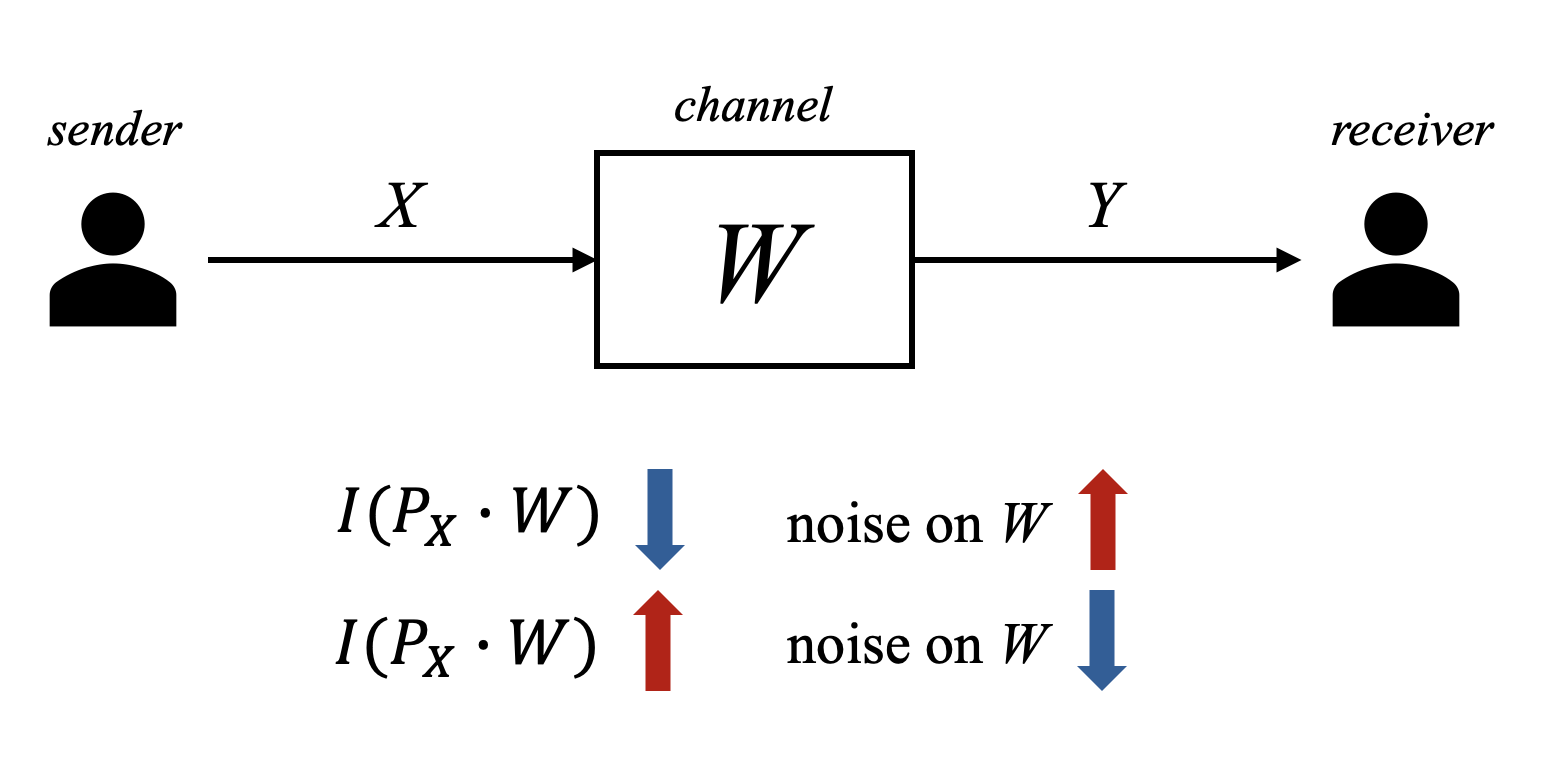
\includegraphics[width=0.55\columnwidth]{image/L2-transmission.png}
                \end{figure}
                \item KL divergence: Hypothesis testing [$\ast$]
                \begin{itemize}
                    \item 어떤 sample space에 대해서 서로 다른 두 hypothesis를 가정해 볼 수 있다.\\ $H_0$: $X \sim P, H_1: X \sim Q$
                    \item $X$를 여러번 관측하여 얻은 realization value를 사용하여얻은 empirical distribution으로부터 실제 probability distribution을 유추할 수 있기 때문에, 어떤 hypothesis가 진실인지 추정할 수 있다.
                    \item Hypothesis testing에서 추정이 틀렸을 확률은 다음과 같이 정의된다.
                    $$P(*) \approx \text{exp}[-n D(P||Q)]$$ 
                    \item 따라서 두 PMF의 KL divergence를 알고있다면 얼마나 많은 데이터($=n$)가 있어야 우리가 원하는 수준의 error-rate를 달성할 수 있는지를 계산할 수 있다.
                    
                \end{itemize}
            \end{itemize}
        \end{frame}
    \end{section}

    %#################################### 
    \begin{section}{Convexity and Concavity of Information Measures}
        \begin{frame}
            \frametitle{Convexity and Concavity}
        
            \begin{definition}[convexity]
                
            \end{definition}
            \begin{definition}[concavity]
                
            \end{definition}
            \begin{itemize}
                \item 
            \end{itemize}
        \end{frame}

        \begin{frame}{Prerequisites: Log-sum inequality}
            \begin{lemma}[log-sum inequality]
                
            \end{lemma}
            
            $\ast$ \underline{Proof}:
        \end{frame}
    
        \begin{frame}
            \frametitle{Convexity of KL-divergence}
            \begin{theorem}
                
            \end{theorem}
            \begin{itemize}
                \item 
            \end{itemize}
            \checkmark \underline{meaning}:
        \end{frame}

        \begin{frame}
            \frametitle{Convexity of KL-divergence}
            $\ast$ \underline{Proof}:
            
        \end{frame}

        \begin{frame}
            \frametitle{Concavity of Entropy}
            \begin{corollary}
                
            \end{corollary}
            \checkmark \underline{meaning}:
            \\ $\ast$ \underline{Proof}: 
        \end{frame}

        \begin{frame}
            \frametitle{Concavity and Concavity of Mutual Information}
            \begin{corollary}
                
            \end{corollary}
            \checkmark \underline{meaning}:
            \\ $\ast$ \underline{Proof}: 
        \end{frame}

        \begin{frame}
            \frametitle{Concavity and Concavity of Mutual Information}
            \begin{corollary}
                
            \end{corollary}
            \checkmark \underline{meaning}:
            \\ $\ast$ \underline{Proof}: 
        \end{frame}

    \end{section}

    \begin{section}{Data Processing Inequality and Fano's Inequality}
        \begin{frame}
            %그림그려서 설명
            \frametitle{Prerequisites: Markov chain}
            \begin{definition}[Markov chain]
            \end{definition}
            \begin{itemize}
                \item 
            \end{itemize}
        
        \end{frame}

        \begin{frame}
            \frametitle{Data Processing Inequality}
            \begin{theorem}[data processing inequality]
                
            \end{theorem}
            \checkmark \underline{meaning}:
            \\ $\ast$ \underline{Proof}: 
        \end{frame}

        \begin{frame}
            \frametitle{Data Processing Inequality}
            \begin{corollary}[Data Processing Inequality on entropy]
                
            \end{corollary}
            \begin{corollary}[Data Processing Inequality on KL-divergence]
                
            \end{corollary}
        \end{frame}
    
        \begin{frame}
            \frametitle{Fano's Inequality}
            \textbf{System}: 
            \begin{theorem}[Fano's inequality]
                
            \end{theorem}
            \checkmark \underline{meaning}:
        \end{frame}

        \begin{frame}
            \frametitle{Fano's Inequality}
            $\ast$ \underline{Proof}: 
        \end{frame}
    \end{section}

    \begin{frame}{Appendix}
        \begin{block}{Notations}
            \begin{itemize}
                \item entropy of r.v. $X \sim P_X$: $H(X), H(P_X)$
                \item conditional entropy of $Y$ conditioned on $X=x$: $H(Y|X=x) , H(P_{Y|X}(\cdot|x))$
                \item conditional entropy of $Y$ conditioned on $X$: $H(Y|X) , H(P_{Y|X})$
                \item mutual information of $X, Y$: $I(X;Y), I(P_X \cdot P_{Y|X}), I(P_X , P_{Y|X})$ \\
                주로 $W= P_{Y|X}$로 두고 $I(P_X \cdot W)$와 같이 표기하여 사용한다.
                \item KL divergence between two distribution $P$ and $Q$: $D(P||Q),  D(P_P||P_Q)$
            \end{itemize}
        \end{block}
    \end{frame}

    \begin{frame}{References}
        \begin{itemize}
            \item T. M. Cover and J. A. Thomas. Elements of Information Theory, Wiley, 2nd ed., 2006.
            \item Lecture notes for EE623: Information Theory (Fall 2024)
        \end{itemize}
        \vspace{6cm}
    \end{frame}

\end{document}